\documentclass{article}
\usepackage{hyperref}
\usepackage[margin=1in]{geometry}
\usepackage{listings}
\usepackage{xspace}
\usepackage{graphicx}

\newcommand{\Gossiper}{\texttt{Gossiper}\xspace}
\newcommand{\Gomat}{\texttt{Gomat}\xspace}
\newcommand{\Go}{\texttt{Go}\xspace}

\begin{document}
    \begin{titlepage}
        \begin{center}
            \Huge\textbf{Gomat specification}\\
            \large\textit{Gauthier Jolly, Kevin Carenou, Matei Oltean}\\
        \end{center}
        \vfill
        \tableofcontents
        \vfill
        \vfill
    \end{titlepage}
    \section{Introduction}
    \Gomat is a tool which allows users to compute complex operation on matrix on a computer network.
    Gomat is in the same time a \texttt{Go API} and a daemon. By running the daemon, a user become part of a network and can use
    the \texttt{Go API} to execute big computation.

    \section{Overview}
    \begin{figure}[!ht]
        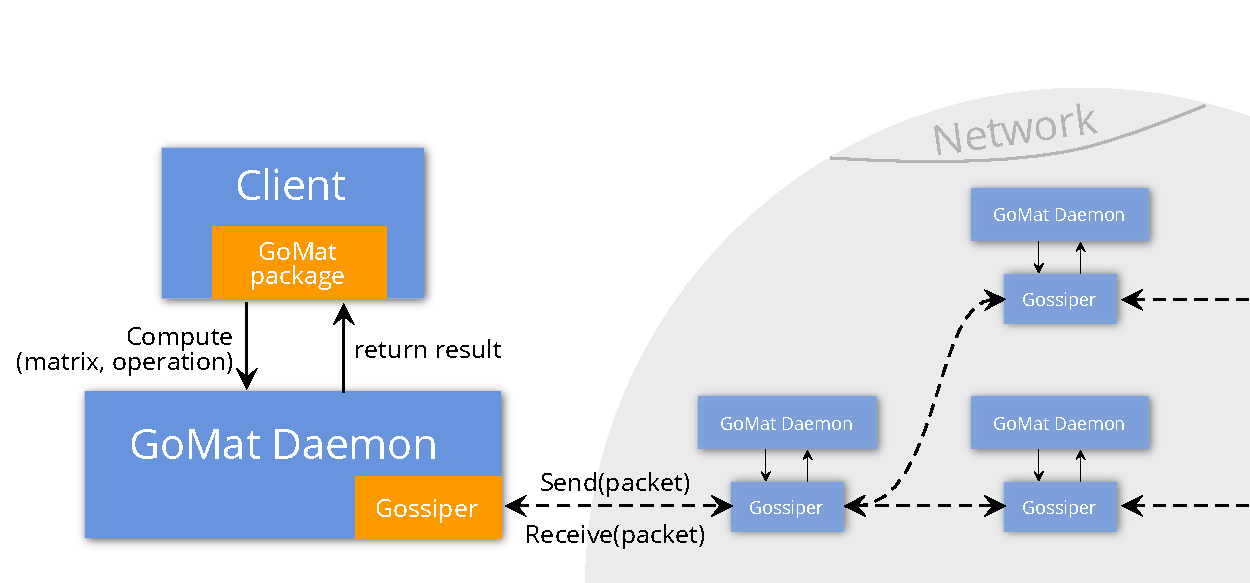
\includegraphics[width=.95\textwidth]{global_view.pdf}
        \caption{Global view}
        \label{glbView}
    \end{figure}
    \begin{figure}[!ht]
        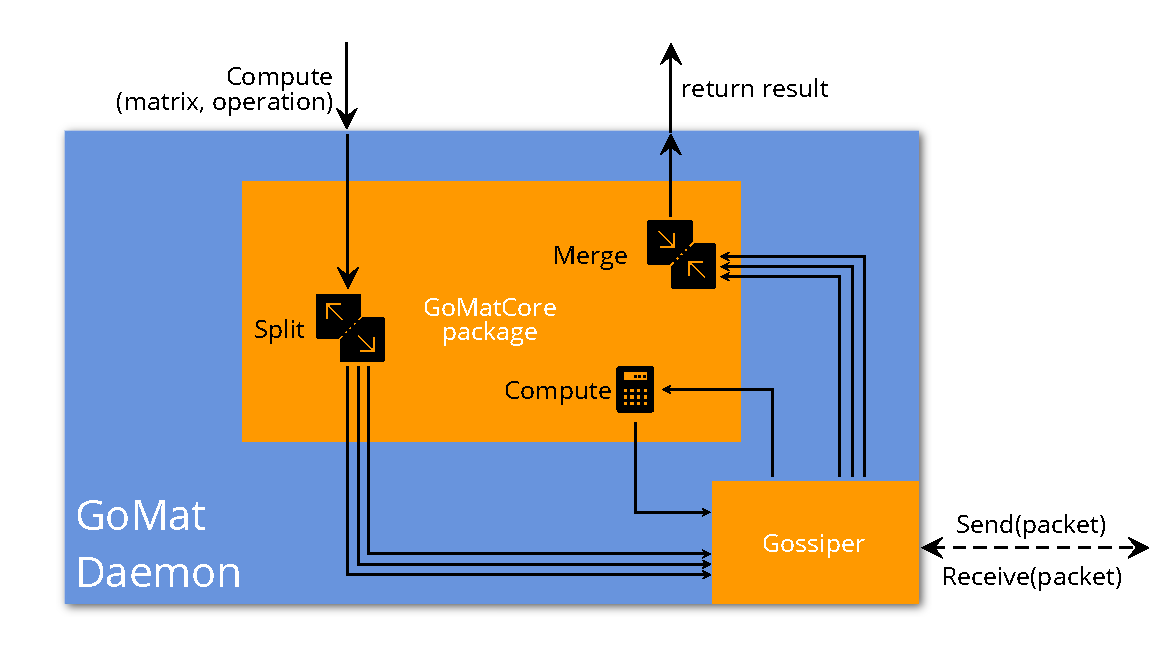
\includegraphics[width=.95\textwidth]{daemon_view.pdf}
        \caption{Daemon architecture}
        \label{daemonView}
    \end{figure}
    \section{Daemon}
    When a user want to join a \Gomat network, he have to run the dedicated daemon. This deamon is the main componant of the
    application. It would split and merge matrices, execute the computations and communicate with other peers. For this last
    point, it uses a \Gossiper network.\\
    A \Gomat peer is not a \Gossiper peer it contains a \Gossiper peer. It uses it to send and receive
    message. Our \Gomat application use the \Gossiper as a transport layer (layer 4).

    \subsection{GUI}
    Once the daemon is running, It is not automaticaly connected to a \Gomat network. The user has to open a web
    browser and go on \url{http://localhost:8080} (can be modify in a configuration file) to add some peers to be connected on a
    \Gomat network.\\
    On the \texttt{GUI}, the client can change the maximum number of computations his computer can do at a time. He can see
    the number of computation his computer have done, check the peers he knows, see our ratio
    ($r = {number of computation tasks sent}/{number of computation tasks computed}$).

    \section{API}
    Our API is a \Go package which is use to speak with our daemon. When a user wants to compute an operation
    between to big matrices, he calls:\\
    \texttt{Gomat.compute(matrix1, matrix2 Matrix, operation Gomat.Operation)(result Matrix, err error)}\\
    This function is blocking.\\
    If there is no \Gomat daemon running on the computer, the Gomat.compute would return an error.
    \subsection{Communications between API and Daemon}
    The API and the Daemon are hosted on the same computer. Thus, there is no need to use the network (i.e. the lo interface).
    We use \texttt{Inter-Process Communication (IPC) sockets} to send information between the daemon and the API.

\end{document}